\documentclass[a4paper,10pt]{article}
\usepackage{geometry}
\usepackage{xcolor}
\usepackage{tcolorbox}
\usepackage{amsmath}
\usepackage{booktabs}
\usepackage{multirow}
\usepackage{tabularx}
\usepackage{graphicx}
\geometry{
    left=1cm,
    right=1cm,
    bottom=2cm,
    top=2cm
}

\usepackage{xepersian}
\settextfont{Vazirmatn-Regular.ttf}

\title{شارا}
\author{شارا}
\date{}

\linespread{1.5}

\begin{document}

    \maketitle

    slide 1 

    در این مطالعه، یک روش‌شناسی برای طراحی معماری سیستم‌های هوش مصنوعی که سازمان‌ها به آن‌ها نیاز دارند، از طریق ساختار IMO شرح داده شده است. روش‌شناسی ما سیستم‌های هوش مصنوعی مورد نیاز و فناوری‌های هوش مصنوعی مورد نیاز را بر اساس فعالیت‌های عملیاتی آینده که توسط سازمان تصور می‌شود، طراحی می‌کند. علاوه بر این، مفهوم ساختار IMO را معرفی کرده‌ایم تا نیازمندی‌های فنی برای توسعه مدل‌های هوش مصنوعی مورد نیاز را شناسایی کند. به عبارت دیگر، روش‌شناسی ما محدودیت‌های مطالعات موجود که فقط نیازمندی‌های سطح انتزاعی را شناسایی می‌کنند را برطرف می‌کند و می‌تواند طراحی را با نیازمندی‌های خاص برای توسعه مدل‌های هوش مصنوعی به صورت عملی مشخص کند. در این بخش، با استفاده از روش‌شناسی ما، مطالعات موردی را توضیح داده و کارایی آن را ارزیابی می‌کنیم.

    slide 2

    به عنوان یک نمونه از روش پیشنهادی، ما یک مثال موردی از یک سیستم ایمنی خودران برای یک وسیله نقلیه مجهز به دو وظیفه هوش مصنوعی ارائه می‌دهیم: جلوگیری از خواب آلودگی راننده و رانندگی خودکار. نتایج نمایش داده شده از طریق خروجی‌های اصلی سه مرحله از روش پیشنهادی ما است: تعریف مسئله، راه‌حل سیستم هوش مصنوعی، و راه‌حل فنی هوش مصنوعی .

    slide 3
    
    \begin{table}[htbp]

        \centering
        \caption{خروجی اصلی مرحله تعریف مشکل برای سیستم پشتیبانی رانندگی ایمن خودمختار برای وسیله نقلیه}
        \begin{tabularx}{\textwidth}{X}

            \hline

            تعریف مسئله \\

            \hline

            [صورت مسئله] \\

            تصادفات رانندگی ناشی از خواب آلودگی هر سال افزایش می‌یابد، و تحلیل روندهای مصرف‌کننده نشان می‌دهد که ترجیح برای خودروهای ایمن در حال افزایش است. در صنعت خودروی آینده به دلیل توسعه فناوری هوش مصنوعی، و به ویژه انتظارات مصرف‌کنندگان با تجربه رانندگی کافی که در افزایش است، تقاضا برای فناوری رانندگی خودکار در آینده در حال افزایش است. \\

            [مشکل باید حل شود] \\

            یک سیستم ایمنی خودکار که می‌تواند رانندگی ایمن برای رانندگان با تجربه کافی نداشته و از رانندگی در حالت خواب‌آلودگی جلوگیری کند، برای نجات یک راننده از تصادفات خودرو لازم است. \\

            \hline

            سناریو(ها) همانطور که هست \\

            \hline

            راننده برای سفر به مقصد «A» وارد خودرو می‌شود و با کنترل شخصی خودرو، از طریق جاده‌های شهری عمومی و کوچه‌ها رانندگی می‌کند. راننده به طرف جلو نگاه می‌کند و فاصله‌ای ایمن از خودروهای اطراف و عابران پیاده را حفظ می‌کند تا از وقوع حوادث جلوگیری کند. \\  

            شرایط $\leftarrow$ زمان $\leftarrow$ روز/شب (24 ساعته) \\
            \hspace{24pt} $\leftarrow$ فضا $\leftarrow$ شهر خیابان/اتوبان \\
            \hspace{24pt} $\leftarrow$ دیگر $\leftarrow$ باران (با بارش 100 میلی‌متر)، برف (با بارش 50 میلی‌متر) \\

            \hline
            
            سناریو(های) آینده \\

            \hline

            راننده برای سفر به مقصد «A» وارد خودرو می‌شود و با کنترل شخصی خودرو، از طریق جاده‌های شهری عمومی و کوچه‌ها رانندگی می‌کند. هنگامی که راننده حالت ایمنی خودرو را فعال می‌کند، خودرو به صورت خودکار حرکات جلوگیری از برخورد را در برابر خودروهای اطراف انجام می‌دهد اگر به آن‌ها نزدیکتر باشند. و هنگامی که خواب‌آلودگی راننده در حالت رانندگی تشخیص داده می‌شود، سیگنال‌های هشدار خواب‌آلودگی بر روی شیشه جلویی خودرو تولید می‌شود و لرزش‌های فرمان تولید می‌شود تا از وقوع تصادفات رانندگی ناشی از خواب‌آلودگی جلوگیری شود. \\

            شرایط $\leftarrow$ زمان $\leftarrow$ روز/شب (24 ساعته) \\
            \hspace{24pt} $\leftarrow$ فضا $\leftarrow$ شهر خیابان/اتوبان \\
            \hspace{24pt} $\leftarrow$ دیگر $\leftarrow$ باران (با بارش 100 میلی‌متر)، برف (با بارش 50 میلی‌متر) \\

            \hline

            نقش(های) هوش مصنوعی \\

            \hline

            \vspace{-10pt}

            \begin{enumerate}
                
                \item هنگامی که موتور روشن است و خواب‌آلودگی راننده تشخیص داده می‌شود (اگر چشمان بیش از 2 ثانیه بسته باشند)، هوش مصنوعی سیگنال‌های هشداری را به شیشه جلویی و فرمان ماشین می‌فرستد.

                \item وقتی راننده حالت ایمن را فعال می‌کند، سپس هوش مصنوعی موقعیت خودروهای اطراف را تشخیص می‌دهد و کنترل خودرو را برای جلوگیری از برخورد کنترل می‌کند.

            \end{enumerate}

            \hrule

        \end{tabularx}
        
    \end{table}

    \newpage

    \lr{slide 4 and 5}
    
    \begin{table}[htbp]
                
        \centering
        \caption{خروجی اصلی مرحله راه حل هوش مصنوعی سیستم برای سیستم پشتیبانی رانندگی ایمن خودمختار برای وسیله نقلیه}

        \vspace{-5pt}

        \begin{tabularx}{\textwidth}{ X }
            
            \hrule

            ماموریت(های) سیستم هوش مصنوعی 

            \vspace{3pt}
            
            \hrule

            \vspace{3pt}

            سیستم پشتیبانی رانندگی ایمن خودرو از رانندگی خواب‌آلود و تصادف خودرو جلوگیری می‌کند. 

            \vspace{3pt}

            \hrule

            \vspace{3pt}

            راه‌حل(های) سیستم هوش مصنوعی 

            \vspace{3pt}

            \hrule

            \vspace{3pt}

            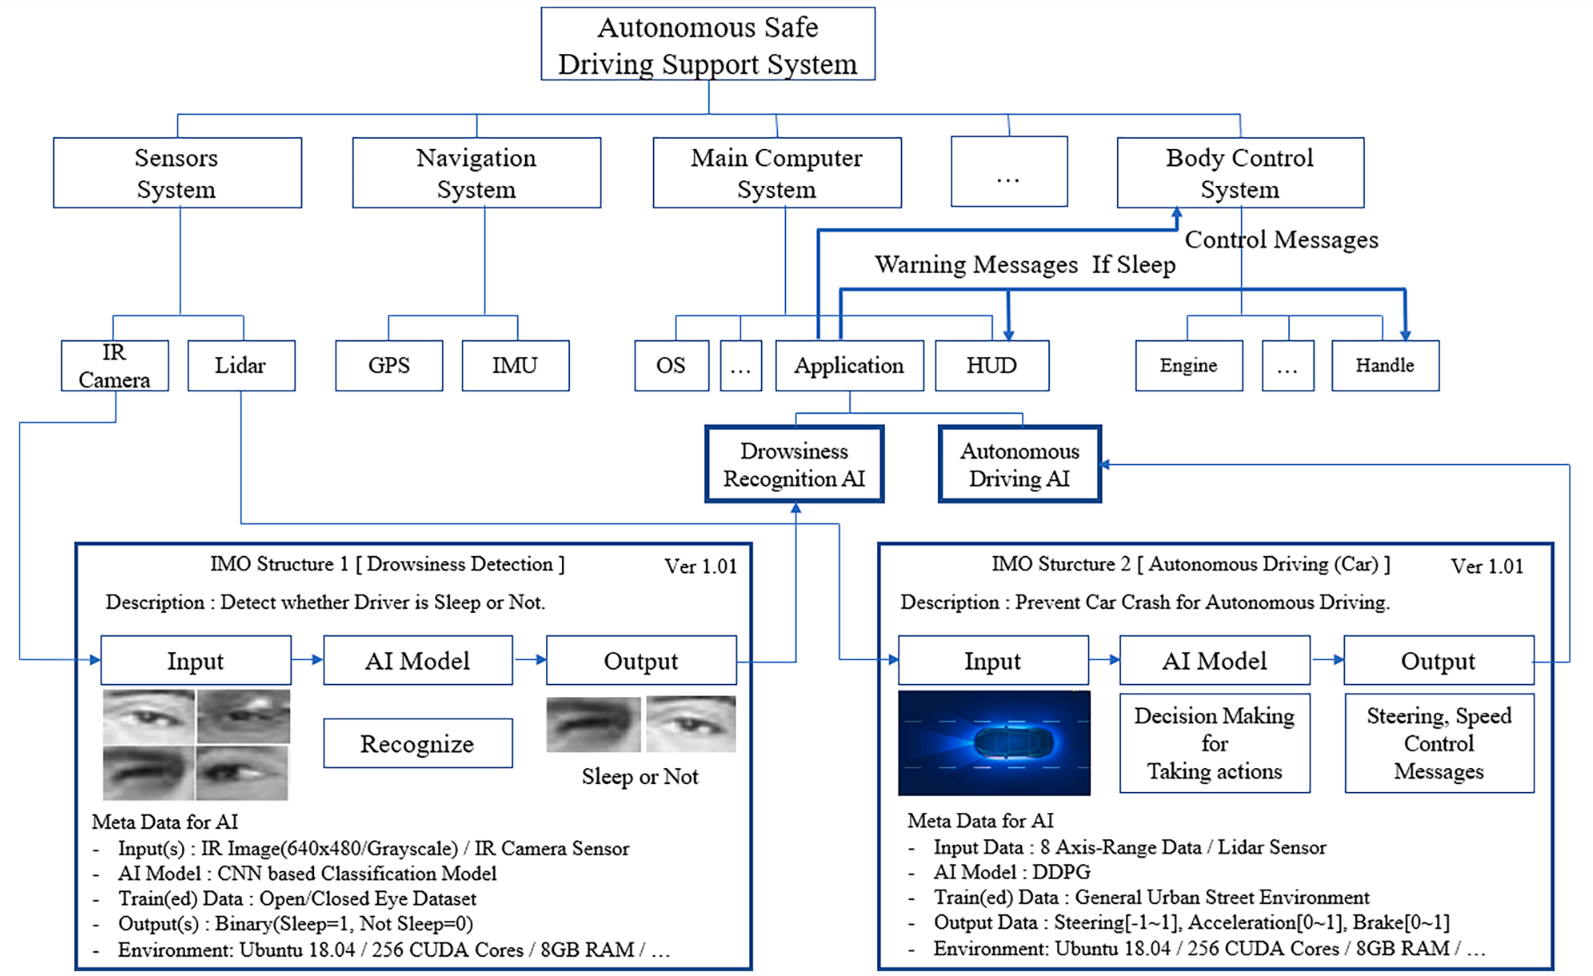
\includegraphics[width=1\linewidth]{image/fig table 5.png} 

            \vspace{3pt}

            \hrule

            \vspace{3pt}

            نیازمندی(های) مولفه(های) هوش مصنوعی

            \vspace{3pt}

            \hrule

            \vspace{3pt}

            جز اصلی سیستم کامپیوتری \\

            \vspace{-10pt}

            \begin{itemize}
                
                \item سیستم‌عامل: 04.18 Ubuntu
                
                \item کارت گرافیک: cores CUDA 256
                
                \item RAM: 8 گیگابایت
                
                \item حافظه: 16 گیگابایت

            \end{itemize}

            \hrule

        \end{tabularx}

    \end{table}

    \newpage

    \lr{slide 6}

    \begin{table}[htbp]

        \centering
        \caption{خروجی اصلی مرحله راه حل فنی هوش مصنوعی برای سیستم پشتیبانی رانندگی ایمن خودمختار برای وسیله نقلیه (هوش مصنوعی تشخیص خواب آلودگی)}
        \begin{tabularx}{\textwidth}{c c c c X}

            \vspace{-10pt}\\

            \hline

            \multicolumn{5}{c}{نقش هوش مصنوعی 1 (هوش مصنوعی تشخیص خواب آلودگی)}\\
            
            \hline

            \multicolumn{5}{c}{راه حل داده}\\

            \multicolumn{1}{c}{I} & \multicolumn{1}{r}{ورودی} & \multicolumn{1}{r}{نوع} &  & تصویر (دوربین مادون قرمز) \\
            & \multicolumn{1}{r}{منبع} & \multicolumn{1}{r}{صفت} &  & 640 $\times$ 480 ، مقیاس خاکستری ، 256 رنگ (قرمز-سبز-آبی) ، 30 فریم بر ثانیه \\
            & \multicolumn{1}{r}{داده/محیط} & \multicolumn{1}{r}{صفت} & \multicolumn{1}{r}{نوع، میزان} & تصویر چشم باز به میزان 5000 عدد، تصویر چشم بسته به میزان 5000 عدد \\
            & \multicolumn{1}{r}{نیازمندی‌ها} &  & \multicolumn{1}{r}{شرایط تفصیلی} & شامل داده هر رنگ پوستی(سفید 33/3\% ، زرد 33/3\% ، سیاه 33/3\%) شامل 50\% داده دارای پوشش عینک (عینک طبی 25\% ، عینک آفتابی 25\%) \\
            & \multicolumn{1}{r}{بنیاد و پایه} & \multicolumn{1}{r}{منبع ورودی} &  & برای دستیابی به نقش هوش مصنوعی، یک سنسور دوربین مادون قرمز و داده های آن که می تواند راننده را در روز/شب در داخل وسیله نقلیه زیر نظر داشته باشد و حتی با یک سنسور به عملکرد دست پیدا کند، مناسب است. \\
            &  & \multicolumn{2}{r}{نیازمندی‌های داده/محیط} & داده‌های مورد نیاز برای یادگیری ویژگی‌ها از ویژگی های مختلف راننده (رنگ پوست، عینک زدن، \dots) تنظیم شده است. \\

            \multicolumn{5}{c}{راه حل تکنیک هوش مصنوعی}\\

            \multicolumn{1}{c}{M} & \multicolumn{1}{r}{مدل هوش مصنوعی} & \multicolumn{2}{c}{نوع} & تشخیص خواب آلودگی \\
            &  & \multicolumn{2}{c}{الگوریتم} & مدل طبقه بندی مبتنی بر CNN \\
            &  & \multicolumn{1}{r}{محیط} & \multicolumn{1}{r}{DEV} & 04.18 Ubuntu / 0.5.2 Tensorflow / 7.3 Python / \dots \\
            &  &  & \multicolumn{1}{r}{OPS} & 04.18 Ubuntu / cores CUDA 256 / 8 گیگابایت RAM / \dots \\
            & \multicolumn{1}{r}{بنیاد و پایه} &  &  & برای دستیابی به نقش هوش مصنوعی، لازم است یک مدل تشخیص برای تشخیص باز یا بسته بودن چشمان راننده اعمال شود. در مقایسه با الگوریتم های مشابه مانند Yolo [23]، یک مدل سبک وزن مبتنی بر CNN که می تواند توابع تشخیص را با محاسبات کم انجام دهد مناسب است. \\

            \multicolumn{1}{c}{O} & \multicolumn{1}{r}{خروجی} & \multicolumn{3}{r}{چشم بسته(1)/باز(0)} \\
            & \multicolumn{1}{r}{عملکرد هوش مصنوعی} & \multicolumn{3}{r}{دقت طبقه‌بندی چشم باز/بسته بیش از 95\%} \\
            & \multicolumn{1}{r}{نیازمندی‌ها} &  &  &  \\
            & \multicolumn{1}{r}{بنیاد و پایه} & \multicolumn{1}{r}{خروجی} &  & برای دستیابی به نقش هوش مصنوعی، لازم است نتایج شناسایی شده ارائه شود، چه چشمان راننده باز یا بسته باشد. \\
            &  & \multicolumn{2}{r}{عملکرد هوش مصنوعی} & با توجه به اهمیت نقش هوش مصنوعی، عملکرد هوش مصنوعی باید تا حد امکان بالا باشد و با توجه به بلوغ تکنولوژیکی الگوریتم‌های مشابه روی بیش از 95\% تنظیم شود [41]. \\
            
            \multicolumn{2}{c}{دلیل نقش هوش مصنوعی} & \multicolumn{3}{r}{نقش 1 هوش مصنوعی که در مرحله تعریف مشکل شناسایی شده است، تشخیص خواب آلودگی راننده و} \\
            \multicolumn{2}{c}{در سیستم مورد علاقه} & \multicolumn{3}{r}{هشدار دادن به هنگام شناسایی خواب آلودگی است. این نقش را می توان با استخراج موقعیت هر چشم} \\
            \multicolumn{2}{c}{} & \multicolumn{3}{r}{از صورت راننده از طریق داده های تصویر دوربین IR و طبقه بندی چشم ها، بسته یا غیر بسته، از طریق} \\
            \multicolumn{2}{c}{} & \multicolumn{3}{r}{ساختار توصیه شده IMO به دست آورد.} \\
            \multicolumn{2}{c}{} & \multicolumn{3}{r}{اگر چشمان راننده بیش از 2 ثانیه بسته باشد (به عنوان مثال، در مورد دوربین 30 فریم بر ثانیه، اگر بیش از} \\
            \multicolumn{2}{c}{} & \multicolumn{3}{r}{60 بار چشمان راننده توسط هوش مصنوعی «بسته» تشخیص داده شود)، به عنوان «خواب آلودگی» در نظر} \\
            \multicolumn{2}{c}{} & \multicolumn{3}{r}{گرفته می شود. در آن زمان، مؤلفه هوش مصنوعی سیگنال‌های هشداری را به HUD واقع در شیشه جلو و} \\
            \multicolumn{2}{c}{} & \multicolumn{3}{r}{فرمان می‌دهد.} \\

            \hline

        \end{tabularx}
        
    \end{table}

    \newpage

    \lr{slide 7}

    \begin{table}[htbp]

        \centering
        \caption{خروجی اصلی راه‌حل فنی هوش مصنوعی سیستم پشتیبانی رانندگی ایمن خودمختار برای وسیله نقلیه (هوش مصنوعی رانندگی خودکار)}
        \begin{tabularx}{\textwidth}{c c c c X}

            \vspace{-10pt}\\

            \hline

            \multicolumn{5}{c}{نقش هوش مصنوعی 2 (هوش مصنوعی رانندگی خودکار)}\\
            
            \hline

            \multicolumn{5}{c}{راه حل داده}\\

            \multicolumn{1}{c}{I} & \multicolumn{1}{r}{ورودی} & \multicolumn{1}{r}{نوع} &  & داده سنسور لیدار \\
            & \multicolumn{1}{r}{منبع} & \multicolumn{1}{r}{صفت} &  & 30 هرتز ، دامنه 0 تا 16 متر \\
            & \multicolumn{1}{r}{داده/محیط} & \multicolumn{1}{r}{صفت} & \multicolumn{1}{r}{نوع، میزان} & محیط مجازی با قابلیت رانندگی بیش از 10000 ساعت با استفاده از حسگر لیدار - * محیط Airsim [42] بر اساس Engine Unreal [43] \\
            & \multicolumn{1}{r}{نیازمندی‌ها} &  & \multicolumn{1}{r}{شرایط تفصیلی} & یک محیط شهری-خیابان/بزرگراه در یک محیط شهری با عابران پیاده با رفتار عادی، وسایل نقلیه اطراف، چراغ های راهنمایی و \dots و می تواند شرایط زیر را بیان کند: روز/شب (24 ساعت)، آفتابی، باران (در عرض 100 میلی متر میزان بارندگی) , برف (در عرض 50 میلی متر میزان بارش برف) \\
            & \multicolumn{1}{r}{بنیاد و پایه} & \multicolumn{1}{r}{منبع ورودی} &  & برای دستیابی به نقش هوش مصنوعی به سنسوری با قابلیت اندازه‌گیری فاصله با دقت بالا نیاز است. از آنجایی که سنسور لیدار بهترین عملکرد را در اندازه گیری فاصله با دقت بالا در بین سایر سنسورهای موجود مانند دوربین فیلمبرداری و رادار نشان می دهد، مناسب است. \\
            &  & \multicolumn{2}{r}{نیازمندی‌های داده/محیط} & یک محیط شهری که در آن یک راننده معمولی می‌تواند رانندگی کند، برای محیط مجازی برای یادگیری هوش مصنوعی مناسب است. \\

            \multicolumn{5}{c}{راه حل تکنیک هوش مصنوعی}\\

            \multicolumn{1}{c}{M} & \multicolumn{1}{r}{مدل هوش مصنوعی} & \multicolumn{2}{c}{نوع} & رانندگی خودکار (جلوگیری از تصادف خودرو) \\
            &  & \multicolumn{2}{c}{الگوریتم} & DDPG \\
            &  & \multicolumn{1}{r}{محیط} & \multicolumn{1}{r}{DEV} & \dots \\
            &  &  & \multicolumn{1}{r}{OPS} & \dots \\
            & \multicolumn{1}{r}{بنیاد و پایه} &  &  & برای دستیابی به نقش هوش مصنوعی، الگوریتم DDPG که می تواند به طور مداوم رفتار خودرو را کنترل کند، مناسب است. \\

            \multicolumn{1}{c}{O} & \multicolumn{1}{r}{خروجی} & \multicolumn{3}{r}{فرمان [1- تا 1+] ، شتاب [0 تا 1] ، ترمز [0 تا 1]} \\
            & \multicolumn{1}{r}{عملکرد هوش مصنوعی} & \multicolumn{3}{r}{تحت شرایط محیط مجازی مشخص شده} \\
            & \multicolumn{1}{r}{نیازمندی‌ها} & \multicolumn{3}{r}{0\% برخورد با وسیله نقلیه یا جسم دیگر (فرد و غیره) در حین رانندگی به مدت 1000 ساعت در 10 بار} \\
            &  & \multicolumn{3}{r}{0\% برخورد هنگام انجام موقعیت های تصادفی وسیله نقلیه و عابر پیاده به تعداد 100 بار} \\
            &  & \multicolumn{3}{r}{(ایست ناگهانی از نزدیک وسیله نقلیه، بریدگی، عبور انسان)} \\
            & \multicolumn{1}{r}{بنیاد و پایه} & \multicolumn{1}{r}{خروجی} &  & برای دستیابی به نقش هوش مصنوعی، هوش مصنوعی باید بتواند فرمان، پدال گاز و ترمز هر وسیله نقلیه را به طور مداوم تنظیم کند. \\
            &  & \multicolumn{2}{r}{عملکرد هوش مصنوعی} & با توجه به اهمیت نقش هوش مصنوعی، عملکرد هوش مصنوعی باید تا حد امکان بالا باشد. برای ارزیابی ایمنی و پایداری هوش مصنوعی، شرایط رانندگی بدون تصادف به ترتیب برای 1000 ساعت در 10 بار در موارد معمول و اضطراری تنظیم شد. برای ارزیابی قابلیت واکنش اضطراری هوش مصنوعی، موقعیت‌های تصادفی تصادفی که شامل برخورد تصادفی وسیله نقلیه با وسایل نقلیه اطراف یا عابران پیاده می‌شود، 100 بار در مواقع اضطراری تنظیم شد. \\
            
            \multicolumn{2}{c}{دلیل نقش هوش مصنوعی} & \multicolumn{3}{r}{نقش 2 هوش مصنوعی شناسایی شده در مرحله تعریف مشکل، جلوگیری از برخورد با سایر وسایل نقلیه و} \\
            \multicolumn{2}{c}{در سیستم مورد علاقه} & \multicolumn{3}{r}{عابران پیاده در صورت روشن بودن حالت ایمن است.} \\
            \multicolumn{2}{c}{} & \multicolumn{3}{r}{این امر توسط هوش مصنوعی وسیله نقلیه که فاصله تا سایر اشیا اطراف خودرو را از طریق حسگر لیدار} \\
            \multicolumn{2}{c}{} & \multicolumn{3}{r}{اندازه‌گیری می‌کند و در صورت تشخیص خطرات برخورد، فرمان و/یا سرعت خودرو را تنظیم می‌کند.} \\

            \hline

        \end{tabularx}
        
    \end{table}

    \newpage

    \lr{slide 8}

    \begin{table}[htbp]
                        
        \centering
        \caption{نتایج تحلیل مقایسه کیفی بین تحقیقات موجود و روش پیشنهادی}
        \begin{tabularx}{\textwidth}{ c X X X }
            
            \hline

            \multicolumn{1}{c}{سوالات} & \multicolumn{1}{r}{اهداف} & \multicolumn{1}{r}{مطالعات موجود} & \multicolumn{1}{r}{روش پیشنهادی} \\

            \hline

            \multicolumn{1}{c}{سوال 1} & شناسایی اهداف پروژه هوش مصنوعی و مفاهیم عملیاتی آینده. & مسائل یا اهمیت مربوط به محتوای هر سؤال مشخص شد، اما هیچ روش مشخصی برای پاسخ به هر سؤال ارائه نشد و رویکرد انتزاعی بود. & ارائه روش های مشخص (خروجی های اصلی مرحله تعریف مسئله) \\
            \multicolumn{1}{c}{سوال 2} & شناسایی سیستمی که مدل هوش مصنوعی در آن مستقر خواهد شد (یا نیاز به استقرار دارد). &  & ارائه روش های مشخص (خروجی های اصلی مرحله حل هوش مصنوعی سیستم) \\
            \multicolumn{1}{c}{سوال 3} & شناسایی الزامات فنی هوش مصنوعی مانند عملکرد و خروجی. &  & ارائه روش های ملموس (خروجی های اصلی مرحله راه حل فنی هوش مصنوعی) \\
            \multicolumn{1}{c}{سوال 4} & شناسایی ملاحظات فنی هوش مصنوعی مانند داده ها، فناوری و غیره. &  & ارائه روش های ملموس (خروجی های اصلی مرحله راه حل فنی هوش مصنوعی) \\
            
            \hline

        \end{tabularx}
        
    \end{table}

    \newpage

    \lr{slide 9}

    \begin{table}
                        
        \centering
        \caption{نتایج تحلیل تطبیقی از منظر طراحی معماری}
        \begin{tabularx}{\textwidth}{ p{4cm} p{9.3cm} c c c c c }

            \hline
            
            \multirow{2}{*}{کارهای مرتبط} & \multirow{2}{*}{نتجه هر مطالعه} & \multicolumn{5}{c}{امتیازات} \\
            &  & Q1 & Q2 & Q3 & Q4 & جمع کل \\
            
            \hline

            تاکدا و همکاران [16] & ارائه نتایج و روش‌شناسی طراحی معماری ربات مبتنی بر هوش مصنوعی مبتنی بر SysML & 2 & 1 & 1 & 2 & 6 \\

            جولیان و جونز و همکاران [17] & طراحی معماری سیستم AMD مبتنی بر DoDAF و شناسایی عملکردهای هوش مصنوعی مورد نیاز & 2 & 1 & 1 & 1 & 5 \\

            کار ما & تعریف مشکل، راه حل هوش مصنوعی سیستم، راه حل فناوری هوش مصنوعی & 2 & 2 & 2 & 2 & 8 \\

            \hline

        \end{tabularx}

    \end{table}

    \newpage

    \lr{slide 10}

    \begin{table}
                        
        \centering
        \caption{نتایج تحلیل بر اثربخشی غلبه بر علل شکست پذیرش هوش مصنوعی سازمانی}
        \begin{tabularx}{\textwidth}{ p{1.5cm} p{6.5cm} c c c c p{5.5cm} }

            \hline

            \multicolumn{1}{c}{مشکلات} & \multicolumn{1}{c}{توضیحات} & \multicolumn{4}{c}{نتایج ارزیابی} & \multicolumn{1}{c}{بنیاد و پایه} \\
            &  & قبل & \multicolumn{3}{c}{روش پیشنهادی} &  \\
            &  & NS & NS & PS & S &  \\
            &  & (0pt) & (0pt) & (1pt) & (2pt) &  \\

            \hline

            اهداف تجاری نامشخص & فقدان اهداف مشخص برای کسب و کارها در مورد اینکه با هوش مصنوعی چه کاری انجام دهند. & V &  &  & V & می توان با استفاده از خروجی های اصلی روش پیشنهادی بر آن غلبه کرد. \\

            رویکرد استراتژیک نادرست & فقدان رویکردها یا فرآیندهای مناسب برای انجام پروژه های هوش مصنوعی. & V &  & V &  & امکان حل تا تحقق هدف پروژه \\

            استراتژی داده ضعیف & عدم توانایی به دست آوردن داده های با کیفیت بالا و مقادیر زیاد مورد نیاز برای هوش مصنوعی. & V &  &  & V & می تواند از طریق خروجی اصلی مرحله 3 غلبه کند. \\

            عدم آگاهی از هوش مصنوعی & مسائل مربوط به اعتماد به دلیل عدم آگاهی اعضای سازمان از فناوری هوش مصنوعی، مانند رد هوش مصنوعی یا اعتقاد کورکورانه به هوش مصنوعی. & V &  &  & V & اعضا می توانند هوش مصنوعی کاربردی را از طریق خروجی های اصلی روش پیشنهادی درک کنند. \\

            فقدان حکمرانی هوش مصنوعی & عدم توانایی نظارت بر تصمیمات یا داده های هوش مصنوعی بر تصمیمات هوش مصنوعی تأثیر می گذارد. & V &  & V &  & می تواند تشخیص دهد که چه چیزی باید از طریق خروجی های اصلی روش پیشنهادی نظارت شود. \\

            عدم استعداد هوش مصنوعی & فقدان استعداد هوش مصنوعی برای رهبری پروژه های هوش مصنوعی (از جمله هوش مصنوعی و تکنسین‌های داده) & V & V &  &  & قابل حل نیست \\

            \hline

            \multicolumn{2}{c}{در مجموع} & 0pt & \multicolumn{3}{c}{8pt از 12pt} \\

            \hline

        \end{tabularx}

    \end{table}

    \newpage

    \lr{slide 11}

    \begin{table}
                        
        \centering
        \caption{اطلاعات کارشناسان شرکت کننده در ارزیابی}
        \begin{tabularx}{\textwidth}{ p{4.5cm} p{5cm} p{6cm} c }
            
            \hline

            \multicolumn{1}{c}{نام} & \multicolumn{1}{c}{سازمان} & \multicolumn{1}{c}{رشته تخصصی} & \multicolumn{1}{c}{دوره‌ها} \\

            \hline

            (P1) M.S.Yang (مهندس ارشد) & تیم نیروی دریایی Systems Hanhwa & توسعه سیستم های رزم دریایی/SW & 25+ سال \\
            (P2) M.W.Lee (دکتری) & ROK DAPA	 & مهندسی نرم‌افزار، فرآیند اکتساب دفاعی & 10+ سال \\
            (P3) J.H.Ahn (ارشد) & وزارت دفاع ملی ROK (تیم آماده سازی مرکز هوش مصنوعی) & برنامه ریزی، مدیریت پروژه هوش مصنوعی & 10+ سال \\
            (P4) J.W.Uhm (دکتری) & ستاد ارتش ROK & مهندسی نرم‌افزار، فرآیند اکتساب دفاعی & 15+ سال \\
            (P5) S.Y.Lee (دکتری) & مدیر ارشد فناوری LG الکترونیک (دفتر ارشد فناوری) & کلان داده، توسعه SW هوش تعبیه شده & 5+ سال \\

            \hline

        \end{tabularx}

    \end{table}

    \newpage

    \lr{slide 12}

    پیشنهادی جدید برای طراحی معماری سیستم‌های هوش مصنوعی براساس یک ساختار IMO به منظور حمایت از انتشار موفق هوش مصنوعی در سازمان‌ها ارائه دادیم. تحقیقات ما فرایند طراحی معماری سیستم موجود را گسترش می‌دهد تا با طراحی فناوری هوش مصنوعی هماهنگ شود. در روش‌شناسی ما، ساختار IMO برای مشخص کردن عملکرد و الزامات فناوری هوش مصنوعی به کار می‌رود. از طریق این رویکرد، ما به طور موثر الزامات برای داده (یا محیط)، الگوریتم‌های هوش مصنوعی و خروجی‌ها، عملکرد هوش مصنوعی و اجزای هوش مصنوعی در فرایند طراحی معماری پیشنهادی شناسایی می‌کنیم. همچنین ما ارزش و محدودیت‌های روش‌شناسی خود را با متخصصان از زمینه‌های مختلف بررسی کرده‌ایم و از طریق این، تأثیرات مثبت مورد انتظار و وظایف تحقیقات اضافی را از دیدگاه هر متخصص در زمینه خود شناسایی کرده‌ایم.

    \newpage
    
    \lr{slide 13}

    روش‌شناسی ما از نظر علمی با ارائه:

        \begin{enumerate}
            
            \item ارائه روشی برای به طور سیستماتیک شناسایی چالش‌های اصلی مانند داده و فناوری هوش مصنوعی که به طور متداول در مطالعات پیشین با هدف موفقیت در انتشار هوش مصنوعی در سازمان‌ها مورد اشاره قرار گرفته‌اند.

            \item ارائه یک روش طراحی معماری سیستم هوش مصنوعی به صورت متمایز و روشن‌تر نسبت به مطالعات قبلی طراحی معماری سیستم که فناوری یا عملکرد مورد نیاز هوش مصنوعی را به صورت انتزاعی شناسایی کردند.

            \item معرفی یک روش‌شناسی که می‌تواند به طور موثر به دلایل اصلی شکست در انتشار هوش مصنوعی که توسط مؤسسات تحقیقاتی معتبر شناسایی شده‌اند، پاسخ دهد.

        \end{enumerate}

    \newpage

    \lr{slide 14}

    همچنین، ما مناطق زیر را برای بهبود کاری که به تحقیقات بیشتری نیاز دارد، شناسایی کرده‌ایم.

    \begin{enumerate}
        
        \item برای اجازه به طراحی معماری در سراسر چرخه عمر مدل‌های هوش مصنوعی، تحقیقات باید گسترش یابد.

        \item نیاز به تجمیع و تحقیقات بیشتر در زمینه بهترین روش‌ها و موازین برای تعریف منطقی عملکرد فناوری‌های هوش مصنوعی است که ممکن است در انواع مختلفی وجود داشته باشند.

    \end{enumerate}


\end{document}